%%%%%%%%%%%%%%%%%%%%%%%%%%%%%%%%%%%%%%%%%%%%%%%%%%%%%%%%%%%%%%%%%%%%%%%%%%%%
%%% 				Customizações do abnTeX2 para o IFCE    			 %%%
%%% 		Instituto Federal de Educação, Ciência e Tecnologia Catarinense %%%
%%%																		 %%%
%%% Template disponível em: https://github.com/clodomirneto/IFCETeX2	 %%%
%%% Desenvolvedores do IFCETeX2: Professor Clodomir Silva Lima Neto		 %%%
%%% 							 Professor Marcelo Araújo Lima			 %%%
%%% E-mails para contato: clodomir.neto@ifce.edu.br						 %%%
%%% 					  marcelo.alima@ifce.edu.br						 %%%
%%%																		 %%%
%%% Agradecimento: Thiago Nascimento 									 %%%
%%% https://github.com/thiagodnf/uecetex2                                %%%
%%%%%%%%%%%%%%%%%%%%%%%%%%%%%%%%%%%%%%%%%%%%%%%%%%%%%%%%%%%%%%%%%%%%%%%%%%%%

%%%%%%%%%%%%%%%%%%%%%%%%%%%%%%%%%%%%%%%%%%%%%%%%%%%%%%%%%%%%%%%%%%%%%%%%%%%%
%%% 						Sequência do GitHub							 %%%
%%%																	     %%%
%%% git status + git add . + git commit + git push					     %%%
%%%%%%%%%%%%%%%%%%%%%%%%%%%%%%%%%%%%%%%%%%%%%%%%%%%%%%%%%%%%%%%%%%%%%%%%%%%%

\documentclass[        
    a4paper,          % Tamanho da folha A4
    12pt,             % Tamanho da fonte 12pt
    chapter=TITLE,    % Todos os capitulos devem ter caixa alta
    %section=TITLE,   % Todas as secoes devem ter caixa alta
    oneside,          % Usada para impressao em apenas uma face do papel
    english,          % Hifenizacoes em ingles
    spanish,          % Hifenizacoes em espanhol
    brazil            % Ultimo idioma eh o idioma padrao do documento
]{abntex2}

% Importações de pacotes
\usepackage[utf8]{inputenc}                         % Acentuação direta
\usepackage[T1]{fontenc}                            % Codificação da fonte em 8 bits
\usepackage{graphicx}                               % Inserir figuras
\usepackage{amsfonts,amssymb,amsmath}               % Fonte e símbolos matemáticos
\usepackage{booktabs}                               % Comandos para tabelas
\usepackage{verbatim}                               % Texto é interpretado como escrito no documento
\usepackage{multirow,array}                         % Múltiplas linhas e colunas em tabelas
\usepackage{indentfirst}                            % Endenta o primeiro parágrafo de cada seção.
\usepackage{listings}                               % Utilizar codigo fonte no documento
\usepackage{xcolor}
\usepackage{microtype}                              % Para melhorias de justificação?
\usepackage[portuguese,ruled,lined]{algorithm2e}    % Escrever algoritmos
\usepackage{algorithmic}                            % Criar Algoritmos  
%\usepackage{float}                                 % Utilizado para criação de floats
\usepackage{amsgen}
\usepackage{lipsum}                                 % Usar a simulação de texto Lorem Ipsum
%\usepackage{titlesec}                               % Permite alterar os títulos do documento
\usepackage{tocloft}                                % Permite alterar a formatação do Sumário
\usepackage{etoolbox}                               % Usado para alterar a fonte da Section no Sumário
%\usepackage[nogroupskip,nonumberlist,acronym]{glossaries}                % Permite fazer o glossario
\usepackage{caption}                                % Altera o comportamento da tag caption
\usepackage[alf,abnt-emphasize=bf,bibjustif, recuo=0cm,abnt-etal-cite=3,abnt-etal-list=0,abnt-etal-text=it]{abntex2cite}  % Citações padrão ABNT
%\usepackage[bottom]{footmisc}                      % Mantém as notas de rodapé sempre na mesma posição
%\usepackage{times}                                 % Usa a fonte Times
\usepackage{mathptmx}                               % Usa a fonte Times New Roman							
%\usepackage{lmodern}                               % Usa a fonte Latin Modern
%\usepackage{subfig}                                % Posicionamento de figuras
%\usepackage{scalefnt}                              % Permite redimensionar tamanho da fonte
%\usepackage{color, colortbl}                       % Comandos de cores
%\usepackage{lscape}                                % Permite páginas em modo "paisagem"
%\usepackage{ae, aecompl}                           % Fontes de alta qualidade
%\usepackage{picinpar}                              % Dispor imagens em parágrafos
%\usepackage{latexsym}                              % Símbolos matemáticos
%\usepackage{upgreek}                               % Fonte letras gregas
\usepackage{appendix}                               % Gerar o apendice no final do documento
\usepackage{paracol}                                % Criar paragrafos sem identacao
\usepackage{ifcetex2}		                        % Biblioteca com as normas do IFCE para trabalhos academicos
\usepackage{pdfpages}                               % Incluir pdf no documento
\usepackage{textcomp}
% Organiza e gera a lista de abreviaturas, simbolos e glossario
%\makeglossaries
% Gera o Indice do documento
%\makeindex

%TEOREMAS

\newtheorem{proposition}{Proposição}[chapter]
\newtheorem{theorem}{Teorema}[chapter]
\newtheorem{lemma}{Lema}[chapter]
\newtheorem{definition}{Definição}[chapter]
\newtheorem{exemplo}{Exemplo}[chapter]
\newtheorem{corollary}{Corolário}[chapter]
\newtheorem{exercicio}{Exercício}[chapter]

%PROVAS

\newenvironment{prova}[1][Prova]{\noindent\textbf{#1.} }{\hfill\rule{0.5em}{0.5em}}
\newenvironment{dem}[1][Demonstra\c c\~ao]{\noindent\textbf{#1.} }{\hfill\rule{0.5em}{0.5em}}
\newenvironment{exm}{\noindent{\textbf{Exemplo:}}}{}

\trabalhoacademico{tccgraduacao}

\ehqualificacao{nao}
\removerbordasdohyperlink{sim} 
% \cordohyperlink{sim}

\autor{Marlon Valmórbida Cendron}
\titulo{A Contribuição das Fases do Sono na Consolidação de Memórias em Redes Neurais de Disparos}
\local{Videira}
\data{2023}

\ies{Instituto Federal de Educação, Ciência e Tecnologia Catarinense}
\iessigla{IFC}
\centro{\textit{Campus} Videira}

% Informação para TCC de Graduação

\graduacaoem{Ciência da Computação} 
\habilitacao{Bacharel} % Licenciado ou Bacharel
\areadeconcentracaograduacao{Ciência da Computação}

% Data de Aprovação

\dataaprovacao{\underline{\hspace*{1cm}}/\underline{\hspace*{1cm}}/\underline{\hspace*{1.2cm}}.}

% Informação sobre o Orientador

\orientador{Prof.\ Dr.\ Manassés Ribeiro}
\orientadories{Instituto Federal de Educação, Ciência e Tecnologia Catarinense}
\orientadoriessigla{IFC}
\orientadorcentro{\textit{Campus} Videira}
\orientadorfeminino{nao} % Coloque 'sim' se for do sexo feminino

\coorientador{} % Deixe o nome do coorientador em branco para remover do documento

% Informação sobre a banca

% Membro da Banca Dois

\membrodabancadois{Prof.\ Dra.\ XXXXX}
\membrodabancadoisies{Instituto Federal de Educação, Ciência e Tecnologia Catarinense}
\membrodabancadoisiessigla{IFC}
\membrodabancadoiscentro{\textit{Campus} Videira}

% Membro da Banca Três

\membrodabancatres{Prof.\ Dra.\ XXXXX}
\membrodabancatresies{Instituto Federal de Educação, Ciência e Tecnologia Catarinense}
\membrodabancatresiessigla{IFC}
\membrodabancatrescentro{\textit{Campus} Videira}

% Informação Complementar sobre a banca

\membrodabancaquatro{Membro da Banca Quatro}
\membrodabancaquatrocentro{Centro de Ciências e Tecnologia — CCT}
\membrodabancaquatroies{Universidade do Membro da Banca Quatro — SIGLA}
\membrodabancacinco{Membro da Banca Cinco}
\membrodabancacincocentro{Teste}
\membrodabancacincoies{Universidade do Membro da Banca Cinco — SIGLA}
\membrodabancaseis{Membro da Banca Seis}
\membrodabancaseiscentro{}
\membrodabancaseisies{Universidade do Membro da Banca Seis — SIGLA}

\begin{document}	

% Elementos pré-textuais

\imprimircapa{}
\imprimirfolhaderosto{}
% %\imprimirfichacatalografica{elementos_pre_textuais/ficha-catalografica}
% %\imprimirerrata{elementos_pre_textuais/errata}
% \imprimirfolhadeaprovacao
% \imprimirdedicatoria{elementos_pre_textuais/dedicatoria}
% \imprimiragradecimentos{elementos_pre_textuais/agradecimentos}
% \imprimirepigrafe{elementos_pre_textuais/epigrafe}
% \imprimirresumo{elementos_pre_textuais/resumo}
% \imprimirabstract{elementos_pre_textuais/abstract}
% \imprimirlistadefiguras
% \imprimirlistadetabelas
% %\imprimirlistadequadros
% %\imprimirlistadealgoritmos
% %\imprimirlistadecodigosfonte
% \imprimirlistadesiglas{elementos_pre_textuais/lista-de-siglas}
% \imprimirlistadesimbolos{elementos_pre_textuais/lista-de-simbolos}
% \imprimirsumario
	
% Elementos textuais

\textual{}
\chapter{Introdução}

A busca pela compreensão e reprodução das habilidades cognitivas e de aprendizado do cérebro humano tem sido um desafio constante
nas áreas de neurociência computacional e Inteligência Artificial (IA). É possível argumentar que as Redes Neurais Artificiais
(RNA) são o mais próximo que já chegamos dessa reprodução; entretanto, as RNAs deixaram de lado o realismo biológico em prol do
aperfeiçoamento da IA~\cite{yamazakiSpiking2022}. As Redes Neurais de Disparos (RND)\footnote{Do inglês \textit{Spiking Neural
Networks}.} representam um avanço significativo em direção ao objetivo de compreender o cérebro humano, uma vez que buscam emular
o comportamento das Redes Neurais Biológicas (RNB) de forma mais realista do que as abordagens tradicionais.

As RNAs convencionais são inspiradas no cérebro: neurônios disparam em determinadas frequências conforme os sinais recebidos de
conexões com outros neurônios através de sinapses plásticas, cuja força muda dinamicamente de acordo com o treinamento.
Entretanto, as semelhanças com o cérebro estão limitadas a este ponto, uma vez que as RNAs tradicionais não capturam a dinâmica
interna dos neurônios biológicos, que disparam de maneiras complexas e distintas, e não apenas em uma determinada frequência.
Outra diferença entre as RNAs e os sistemas biológicos é que elas possuem um período de treinamento em que as sinapses são
otimizadas, e um período em que não há mais treinamento e as sinapses se tornam estáticas; enquanto que nas RNBs as sinapses estão
sempre se alterando conforme a experiência, salvo nos raros casos em que há um período crítico de aprendizado durante a infância,
que é desativado quando o indivíduo se torna adulto~\cite{crepelRegression1982}.

As RNDs são modelos muito mais próximos das RNBs que se comunicam por meio de impulsos elétricos discretos, chamados de disparos,
e que aprendem por métodos realistas, como a plasticidade das sinapses. O grau de realismo biológico de uma RND depende de sua
implementação, podendo empregar modelos de neurônios tão simples quanto uma única equação, que descreve a mudança de tensão
elétrica de um neurônio~\cite{burkittReview2006}, ou até modelos que simulam canais de íons~\cite{hodgkinQuantitative1952},
ramificações de dendritos~\cite{pagkalosIntroducing2023}, entre outros. As RNDs não só representam uma possível evolução das RNAs,
como também são usadas para seu propósito original: compreender o cérebro através da simulação.

A principal característica que torna as RNAs capazes de aprender é seu método de retropropagação de erro, um método de treinamento
que até pode existir em alguns casos no cérebro~\cite{lillicrapBackpropagation2020,songCan2020}, mas que é diferente da forma de
aprendizado local por plasticidade das RNBs~\cite{yamazakiSpiking2022}.

No entanto, treinar RNDs continua sendo uma tarefa desafiadora, já que os algoritmos de aprendizado empregados nas RNAs, além de
não serem biologicamente realistas, também não são diretamente aplicáveis às RNDs devido à natureza discreta dos disparos que as
torna não diferenciáveis, impedindo o cálculo de gradientes, parte fundamental no treinamento de RNAs.

O principal método empregado para o aprendizado de RNDs é a plasticidade das sinapses. A plasticidade é a capacidade do cérebro de
se adaptar e reorganizar suas conexões neurais em resposta a novas informações, experiências ou estímulos; é a principal
propriedade por trás do aprendizado e da formação de memórias. Uma das principais formas de plasticidade neural foi primeiramente
descrita por~\cite{hebbOrganization1949}, chamada de plasticidade hebbiana e influenciada pelas ideias
de~\cite{santiagoCroonian1894}, que pode resultar no fortalecimento ou enfraquecimento das sinapses com base na ativação
simultânea de neurônios conectados: caso o neurônio pós-sináptico dispare logo após o neurônio pré-sináptico, significa que há uma
correlação entre eles e a sinapse é fortalecida, caso contrário, a sinapse é enfraquecida.

A plasticidade hebbiana, resumida pela expressão ``neurônios que disparam juntos, conectam-se juntos'', descreve a formação de
conjuntos celulares\footnote{Do inglês \textit{Cell Assemblies}. Também traduzido como Assembleias Celulares.} como resultado do
fortalecimento das conexões entre neurônios ativados simultaneamente. Esses conjuntos podem funcionar como mecanismos de memória
associativa~\cite{sakuraiMultiple2018}. Tomando como exemplo a memória de uma viagem à praia: essa memória consiste em vários
elementos, como o som das ondas, a sensação de areia sob os pés, o cheiro de água salgada, a visão do mar, entre outros. Cada um
desses elementos sensoriais é processado em diferentes áreas do cérebro e ativa diferentes grupos de neurônios. A ativação
síncrona dos neurônios responsáveis por esses elementos sensoriais leva à formação de um conjunto celular. Algum tempo depois, ao
sentir o cheiro do mar novamente, esse estímulo pode acabar ativando o conjunto celular, resultando na experiência da memória.
Conjuntos celulares não são estruturas estáticas, essas redes dinâmicas de neurônios que surgem a partir da experiência estão
sujeitas a modificações e reativações ao longo do tempo, sendo influenciadas pela falta de estímulos ou novas informações, o que
pode levar à alteração ou esquecimento de partes da memória.

A plasticidade hebbiana, no entanto, não consegue gerar, por si só, conjuntos celulares estáveis quando simulada em uma RND;\@
isso ocorre pois a atividade neural continuamente modifica as sinapses, fazendo com que em pouco tempo quaisquer estímulos não
relacionados com a informação codificada no conjunto celular acabem alterando as sinapses e desfazendo o conjunto
celular~\cite{gerstnerSpiking2002}.

Mas a plasticidade hebbiana não descreve toda a gama de diferentes modos com que a plasticidade se manifesta no cérebro, como é o
caso das  plasticidades heterossináptica, em que a ativação de neurônios causa mudanças em neurônios inativos, e homeostática, um
processo lento em que as sinapses se auto-regulam para garantir estabilidade. A plasticidade também depende do tipo de neurônio,
do tipo da conexão, do tempo de efeito das alterações (curto ou longo-prazo), entre outros fatores. A natureza do efeito da
plasticidade também varia muito, podendo depender da frequência de disparos, da diferença de potencial, do tempo dos disparos,
entre outros. Nas RNDs, assim como ocorre com os modelos de neurônios, os modelos de plasticidade também possuem uma ampla
variação em termos de plausibilidade biológica. Além disso, dependendo do modelo que se deseja utilizar, pode-se combinar
múltiplos modelos de plasticidade simultaneamente. Uma RND com plasticidade hebbiana junto de outras formas de plasticidade é
capaz de formar conjuntos celulares estáveis por horas~\cite{zenkeDiverse2015}.

O sono é um processo fisiológico crucial para a consolidação\footnote{A consolidação de uma memória é entendida como o processo
que transforma novas memórias frágeis criadas enquanto acordado para memórias mais estáveis e de longo prazo} e manutenção das
memórias~\cite{blissittSleep2001, walkerSleep2006, diekelmannMemory2010}. Inicialmente, postulava-se que o sono desempenhava uma
função passiva no processo de consolidação da memória~\cite{jenkinsObliviscence1924}; contudo, com a descoberta das distintas
fases do sono, começaram-se a explorar as contribuições ativas do sono na consolidação mnemônica~\cite{aserinskyRegularly1953}.
Durante o sono, ocorrem diferentes fases caracterizadas por padrões distintos de atividade cerebral: sono REM (\textit{Rapid Eye
Movement}) e sono não REM (NREM, dividido entre as fases N1, N2 e N3)~\cite{schulzRethinking2008}. Durante a fase NREM, oscilações
lentas, fusos e ondulações coordenam a reativação e redistribuição de memórias dependentes do hipocampo para o
neocórtex~\cite{diekelmannMemory2010}. Já quanto ao sono REM, a dificuldade em isolar a atividade neural dessa etapa específica,
que ocorre após a fase NREM, torna a discussão sobre sua contribuição para a consolidação da memória ainda controversa. Contudo,
pesquisas mais recentes oferecem evidências de que o sono REM desempenha um papel fundamental na consolidação da memória espacial
e contextual~\cite{boyceREM2017}.

Neste contexto, o problema a ser abordado neste trabalho consiste em explorar a retenção de memórias em uma RND.\@ A principal
hipótese a ser avaliada neste trabalho é de que abordagens baseadas em simulações de fases do sono podem melhorar a estabilidade
de conjuntos celulares contribuindo para o processo de retenção de memórias.

\section{Objetivo geral}

O objetivo geral consiste em desenvolver simulações das diferentes fases do sono em RNPs, analisando como a consolidação e
retenção de memórias da rede pode ser afetada.


\section{Objetivos específicos}

Para melhor entendimento do objetivo geral, os seguintes objetivos específicos são propostos:

\begin{itemize}

  \item Investigar as características e propriedades das diferentes fases do sono para criar uma base sólida para a simulação das
das mesmas em uma RND.\@

  \item Estudar e selecionar o modelo de RND mais apropriado para a simulação das fases do sono, levando em consideração a
capacidade de representar a atividade neural durante o sono e a flexibilidade para incorporar diferentes mecanismos de
consolidação de memória.

  \item Sugerir e validar métodos para avaliar a consolidação e retenção de memórias na RND a fim de comparar a performance da
  RND com e sem a simulação do sono.

  \item  Analisar os resultados da simulação para identificar como a consolidação e retenção de memórias são afetadas pelas
diferentes fases do sono e pela atividade neural durante essas fases.

  \item Contribuir para o entendimento dos mecanismos subjacentes aos processos de aprendizado e memória no cérebro, assim como
discutir possíveis implicações e aplicações nos campos de neurociência computacional e inteligência artificial.

\end{itemize}




\chapter{Fundamentação teórica}

\section{Neurônios biológicos}

Neurônios são células especializadas que atuam como unidades básicas de comunicação no cérebro, transmitindo informações através
de impulsos elétricos e conexões químicas e elétricas, chamadas sinapses. Um neurônio possui três principais partes: dendritos,
soma e axônio. Dendritos recebem sinais de outros neurônios e os conduzem ao soma, onde são integrados. Se o sinal integrado
atinge um limiar, um potencial de ação, ou disparo, é gerado no axônio, propagando-se até as terminações axonais através das
sinapses, onde o sinal se propaga para os dendritos dos neurônios seguintes.

<imagem de um neurônio>

O potencial de membrana é o potencial elétrico interior da célula em relação ao exterior. Em repouso, um neurônio possui um
potencial de membrana negativo, de -40mV a -80mV, chamado potencial de repouso, que é mantido através da bomba de sódio-potássio e
da permeabilidade seletiva da membrana. Em vários neurônios, uma despolarização de aproximadamente 10mV é o suficiente para
atingir o limiar de excitação, que, uma vez atingido, desencadeia a abertura dos canais de sódio (Na+) voltagem-dependentes,
permitindo a entrada de mais Na+ e causando uma maior despolarização. Quando o potencial de membrana
atinge seu pico, normalmente por volta de +40mV, os canais de Na+ se fecham, enquanto os canais de potássio (K+)
voltagem-dependentes se abrem, permitindo a saída de K+ e repolarizando a membrana. Esse processo é seguido por uma
hiperpolarização temporária, antes que o potencial de membrana retorne ao seu estado de repouso. Essa sequência de eventos
constitui um potencial de ação, que se propaga ao longo do axônio até as sinapses, permitindo a comunicação entre os
neurônios~\cite{kandelPrinciples2021}.

\begin{figure}[!ht]
\Caption{Potencial de ação, linha vermelha, condutância da membrana, envelope.}
\centering
\label{action_potential}
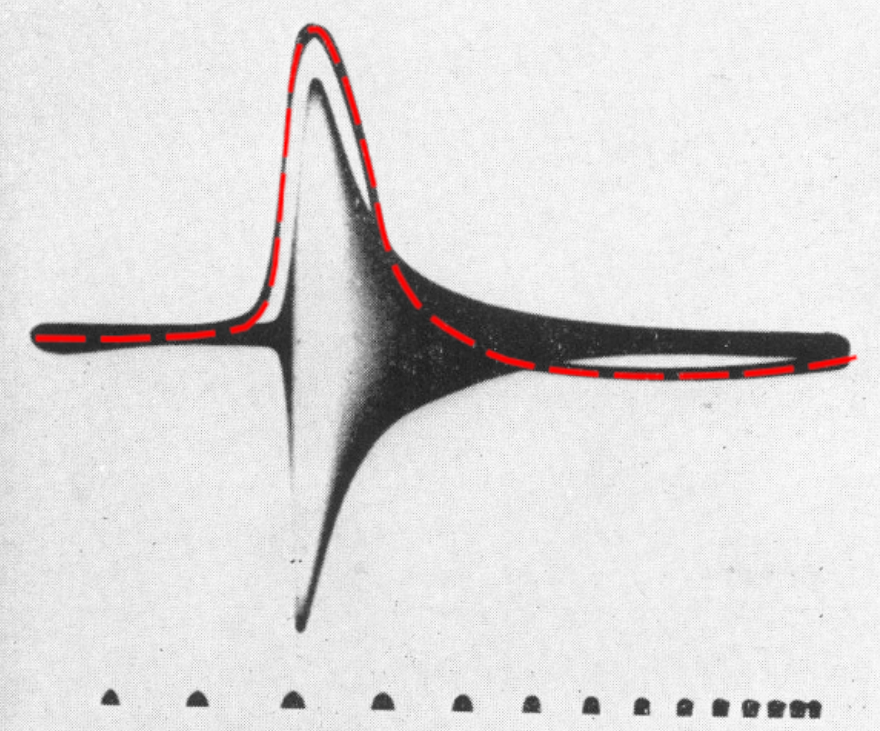
\includegraphics[width=8.5cm]{figuras/Action Potential.png}
\Fonte{Fonte.}
\end{figure}

% Imagem daqui: https://core.ac.uk/download/pdf/82621126.pdf
% Eu adicionei a linha vermelha
% Original por coleELECTRIC1939

As sinapses podem ocorrer de duas maneiras distintas: por meio de transmissão química, utilizando neurotransmissores, ou por
transmissão elétrica. Embora a transmissão química seja mais lenta, ela pode intensificar o sinal transmitido, enquanto a
transmissão elétrica é mais rápida, mas não é capaz de modificar a amplitude do sinal. As sinapses podem ter um efeito
excitatório, resultando em despolarização da célula pós-sináptica, ou um efeito inibitório, resultando em hiperpolarização. Entre
os neurotransmissores mais comuns que causam efeito excitatório estão o glutamato, a dopamina e a noradrenalina, enquanto o GABA,
a glicina e a serotonina são exemplos de neurotransmissores que exercem efeito inibitório.

Quando um potencial de ação chega à terminação axonal do neurônio pré-sináptico, vesículas contendo neurotransmissores são
liberadas na fenda sináptica. Os neurotransmissores se ligam a receptores específicos na membrana do neurônio pós-sináptico,
ativando ou inibindo os canais iônicos. Se o neurotransmissor for excitatório, ele induz a abertura de canais iônicos como os de
Na+ e Ca2+, resultando em uma entrada líquida de íons positivos e uma despolarização da membrana pós-sináptica. Por outro lado, se
o neurotransmissor for inibitório, ele geralmente causa a abertura de canais de K+ e/ou Cl-, levando à saída de íons K+ ou entrada
de íons Cl-, o que resulta em uma hiperpolarização da membrana pós-sináptica.

\section{Modelos de Neurônios}\label{section_modelos_neuronios} 

Em 1907, Lapicque desenvolveu um modelo de neurônio que descreve o neurônio como um circuito elétrico contendo um capacitor e um
resistor em paralelo, como representado na Figura~\ref{fig_lapicque}, representando a capacitância e a resistência de vazamento da
membrana celular~\cite{lapicqueRecherches1907}, chamado de modelo Integrate-and-Fire (IF). Mesmo sem entender os mecanismos por
trás da geração de potenciais de ação, Lapicque postulou que, ao atingir um certo potencial limiar, um potencial de ação seria
gerado e o capacitor descarregado, reiniciando o potencial da membrana. Isso mostra que, ao se tratar de modelagem de neurônios,
estudos da função não necessariamente requerem conhecimento do mecanismo~\cite{abbottLapicque1999}. O modelo de neurônio de
Lapicque foi a primeira tentativa de representar matematicamente um neurônio biológico.

\begin{figure}[!ht]
\caption{(A) O circuito elétrico de Lapicque: I é a corrente injetada, C a capacitância da membrana, R a resistência da membrana,
V o potencial de membrana e $V_{rest}$ o potencial de repouso. (B) A trajetória de tensão, quando um limiar é atingido, um
potencial de ação é disparado. (C) Um modelo IF com corrente que varia pelo tempo.}
\centering{
\parbox{\linewidth}{
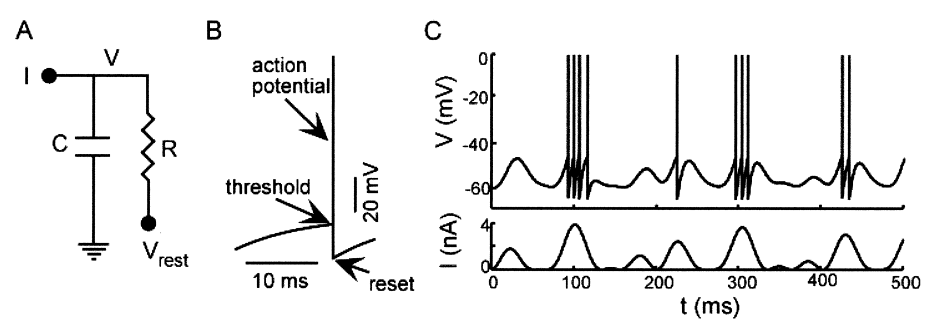
\includegraphics[width=\linewidth]{figuras/lapicque.png}\label{fig_lapicque}
\fonte{\citeonline{abbottLapicque1999}.}}}
\end{figure}

O modelo de Hodgkin-Huxley~\cite{hodgkinQuantitative1952}, representou um a\-van\-ço significativo na compreensão e na modelagem dos
neurônios biológicos. Diferentemente do primeiro modelo criado por Lapicque, esse modelo buscou descrever a geração e propagação
de potenciais de ação em neurônios levando em consideração os processos eletroquímicos subjacentes, como a dinâmica dos diferentes
canais iônicos que controlam a corrente elétrica através da membrana celular.

O modelo de Hodgkin-Huxley é composto por um conjunto de equações diferenciais ordinárias que descrevem a variação do potencial de
membrana em função do tempo e das correntes iônicas. Essas equações consideram o comportamento dinâmico dos canais iônicos de
sódio e potássio, bem como a corrente de vazamento através da membrana. O modelo é capaz de capturar o comportamento típico dos
neurônios, incluindo a resposta ao estímulo, a fase refratária e a propagação do sinal ao longo do axônio.

Baseados na ideia de Lapicque, hoje em dia são utilizados os modelos IF.\@ Existem diversos modelos IF, com
várias modificações da ideia original, como o modelo Leaky Integrate-and-Fire (LIF)~\cite{burkittReview2006}. Os modelos IF são
uma alternativa mais simples e computacionalmente eficiente em comparação ao modelo de Hodgkin-Huxley. Embora não sejam tão
biologicamente precisos quanto o modelo de Hodgkin-Huxley, os modelos IF conseguem capturar algumas das características essenciais
dos neurônios, como a integração temporal dos estímulos e a emissão de potenciais de ação quando um limiar é atingido. Outra
vantagem dos modelos IF é que modelos simples são uma forma de reduzir a complexidade do cérebro para seus mecanismos mais
fundamentais.

Devido a sua simplicidade, os modelos IF têm sido amplamente utilizados em RNP pela sua eficiência computacional e capacidade de
reproduzir aspectos fundamentais do comportamento neuronal. Por exemplo, no trabalho de~\citeonline{teeterGeneralized2018} o
comportamento de 645 neurônios do neocórtex foi reproduzido utilizando modelos GLIF (Generalized Leaky Integrate-and-Fire). 

O modelo de neurônio LIF é descrito pela dinâmica do potencial de membrana do neurônio, $v(t)$, que é dado pela
Equação~\ref{eq_lif} e uma condição adicional para a geração de potenciais de ação, dada pela Equação~\ref{eq_lif_cond}:

\begin{equation}
\label{eq_lif}
C_m \frac{d}{dt}v(t) = -\frac{C_m}{\tau_m} [v(t) - V_0] + I(t)
\end{equation}

\begin{equation}
\label{eq_lif_cond}
\text{se}\quad v \ge v_{th} \quad \text{então} \quad v \gets v_{reset}
\end{equation}

\noindent{}onde $C_m$ é a capacitância da membrana, $V_0$ é o potencial de repouso, $\tau_m$ é a constante de tempo passiva da membrana
(relacionada à capacitância do neurônio e à resistência de vazamento do potencial de membrana por $\tau_m = R_m C_m$), $I(t)$ é a
corrente elétrica injetada no neurônio (tanto a corrente causada pelas sinapses, como a por eletrodos)~\cite{burkittReview2006}. 

Quando o potencial de membrana atinge um limiar, $V_{th}$, um potencial de ação é disparado e o potencial de membrana retorna
para $V_{reset}$, o potencial um pouco menor que o potencial de repouso, correspondente ao período refratário do neurônio.

Existem diversos outros modelos de neurônios, como o modelo de Izhikevich~\cite{izhikevichSimple2003}, que é quase tão simples em
termos computacionais quanto o modelo IF, mas que consegue capturar de forma muito mais realista um conjunto maior de
comportamentos neurais dependendo dos parâmetros utilizados, como mostra a Figura~\ref{fig_izhikevich}.

\begin{figure}[!ht]
\caption{Diferentes tipos de neurônios simulados pelo modelo de Izhikevich.}
\centering{
\parbox{\linewidth}{
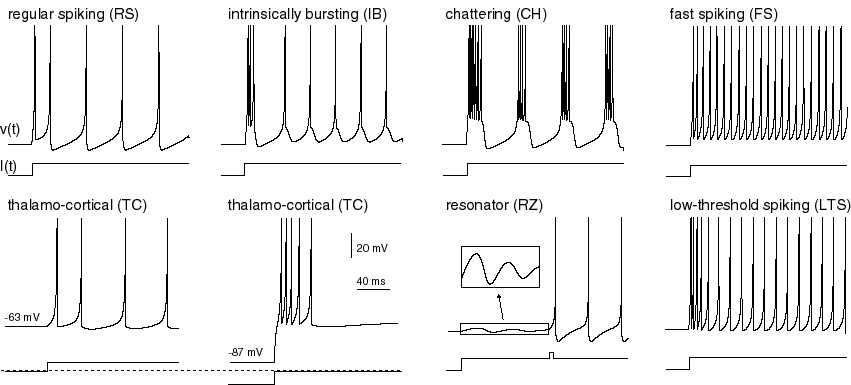
\includegraphics[width=\linewidth]{figuras/izhikevich.png}\label{fig_izhikevich}
\fonte{\citeonline{izhikevichSimple2003}.}}}
\end{figure}

O modelo de Izhikevich é especialmente útil quando se deseja estudar populações de neurônios específicos do cérebro. Já os modelos
IF, como o modelo LIF escolhido para ser utilizado neste trabalho, são preferidos quando o objetivo é estudar o comportamento
geral de neurônios por conta de sua simplicidade.

\subsection{Modelos de Sinapses}\label{subsection_modelos_sinapses}

Para modelar a comunicação entre neurônios, é necessário modelar as sinapses. Existem diversos modelos de sinapses, que variam em
complexidade e precisão. O modelo mais simples e muito utilizado é o modelo de sinapse de condução, que é uma sinapse estática,
que não possui plasticidade e não se adapta ao longo do tempo. A dinâmica de condutância\footnote{A condutância é o inverso da
resistência.} da sinapse é descrita pela Equação~\ref{eq_sinapse}:

\begin{equation}
\label{eq_sinapse}
\frac{d}{dt}g_{syn}(t) = \bar{g}_{syn}\sum_{k}{\delta(t-t_k)} - g_{syn}(t)/\tau_{syn}
\end{equation}

\noindent{}onde $g_{syn}(t)$ refere-se à condutância da sinapse, $\bar{g}_{syn}$ é a condutância máxima da sinapse, ou o peso da
sinapse, que determina o quão forte é a influência da sinapse no neurônio pós-sináptico, $\delta(x)$ é a função delta de Dirac, que
vale 1 quando $x=0$ e 0 caso contrário, esse somatório resulta em 0 caso não tenha havido nenhum potencial de ação na sinapse no
tempo $t$.

A lei de Ohm\footnote{Dada por $V=IR$, onde a tensão é igual à corrente elétrica multiplicada pela resistência.} é utilizada para
calcular a corrente elétrica a partir da condutância da sinapse, que é dada pela Equação~\ref{eq_sinapse_curr}:

\begin{equation}
\label{eq_sinapse_curr}
I_{syn}(t)=g_{syn}(t)(V(t)-E_{syn})
\end{equation}

\noindent{}onde $V(t)$ é o potencial da membrana e $E_{syn}$ corresponde ao potencial de reversão da sinapse, que determina se a sinapse é
excitatória ou inibitória.



\section{Modelos de Plasticidade}

https://compneuro.neuromatch.io/tutorials/W2D3_BiologicalNeuronModels/student/W2D3_Tutorial3.html


A plasticidade é um conceito chave na neurociência e se refere à capacidade dos neurônios de modificar suas sinapses e
comportamento em resposta a experiências e estímulos. Modelos de plasticidade incluem:

STP, STP, STDP, Homeostática, etc.



\section{Redes Neurais de Disparos}

\section{Conjuntos Celulares}

A plasticidade dá origem a um fenômeno emergente no cérebro chamado de conjuntos celulares, fenômeno em que grupos de neurônios
relacionados a um mesmo estímulo ou processo acabam fortalecendo as conexões entre si e que podem servir diversas funções, como
pequenas unidades de processamento, memória associativa, entre outras.

\begin{figure}[!ht]
\centering\label{fig_conjunto_celular}
\Caption{Esquerda: Rede neural sem memórias. Direita: Rede neural com um conjunto celular formado pela experiência.}
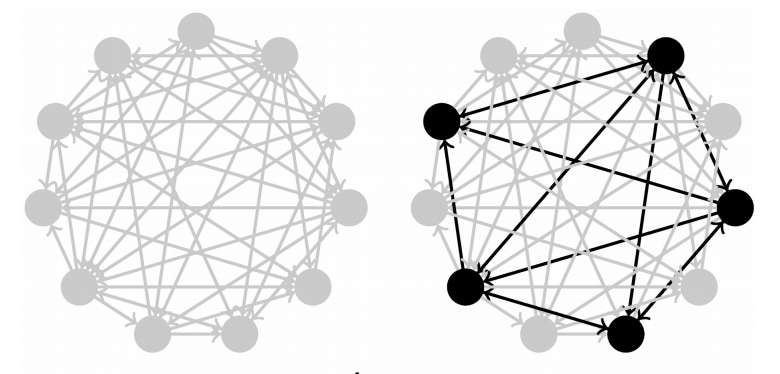
\includegraphics[width=8.5cm]{figuras/Conjunto celular.png}
\Fonte{\cite{zenkeDiverse2015}}
\end{figure}

Tomando um exemplo simplificado da memória de uma viagem à praia: essa memória consiste em vários elementos, como o som das ondas,
a sensação de areia quente, o cheiro de água salgada e a visão de gaivotas etc. Cada um desses elementos sensoriais é processado
em diferentes áreas do cérebro e ativa diferentes grupos  de neurônios. No momento da formação da memória, os neurônios ou grupos
de neurônios responsáveis por esses elementos sensoriais disparam ao mesmo tempo, criando uma correlação entre eles. Essa
correlação é o que desencadeia a plasticidade, esses neurônios terão então as conexões entre si fortalecidas. Com a memória
formada, em um momento futuro em que o indivíduo com a memória ouça novamente o som das ondas, por exemplo, por conta da agora
forte conexão dos neurônios do estímulo sonoro das ondas com as demais características da memória codificada no conjunto celular,
é possível que os neurônios relacionados com a sensação da areia, com o cheiro da água etc.\ também sejam ativados, resultando
então na experiência da memória.

O exemplo dado no parágrafo anterior é bem simplificado, servindo apenas para entender como funciona a formação de conjuntos
celulares e a sua relação com as memórias. O cérebro humano é muito mais complexo e possui muito mais neurônios, não
necessariamente vai haver uma conexão direta entre um neurônio que ativa para o conceito de ondas e um neurônio que ativa para o
conceito de areia, por exemplo, muitas vezes nem existe um neurônio único ou um grupo de neurônios específicos que delimitam o
conceito no cérebro; também, a formação de memórias no cérebro não ocorre apenas pelo simples funcionamento da plasticidade,
embora esse seja o mecanismo por trás de tudo, no cérebro existem áreas específicas que mediam a formação de memórias, como o
hipocampo por exemplo, que possui como uma de suas funções conhecidas a de repetir diversas vezes estímulos no córtex de modo a
fixar memórias de longo prazo~\cite{guptaHippocampal2010}.


\section{Sono}

O sono é um processo fisiológico crucial para a consolidação e manutenção das memórias~\cite{blissittSleep2001, walkerSleep2006,
diekelmannMemory2010}. Inicialmente, postulava-se que o sono desempenhava uma função passiva no processo de consolidação da
memória~\cite{jenkinsObliviscence1924}; contudo, com a descoberta das distintas fases do sono, começaram-se a explorar as
contribuições ativas do sono na consolidação mnemônica~\cite{aserinskyRegularly1953}.

O sono possui 5 fases no total, ilustradas na Figura~\ref{fig_fases}, diferenciadas por suas características distintas de
atividade elétrica cerebral, conforme medido por eletroencefalogramas (EEG)\cite{silberVisual2007}: vigília (acordado), N1, N2, N3
e REM (\textit{Rapid Eye Movement}).\@As fases N1 a N3 são conhecidas como sono não-REM (NREM). Ao cair no sono, a fase N1 é a
primeira a ser atingida, seguida por N2, N3, N2 novamente e, por fim, REM;\@esse ciclo se repete ao longo da noite, com cada ciclo
durando aproximadamente de 90 a 110 minutos~\cite{k.patelPhysiology2022}.

\begin{figure}[!ht]
\Caption{\label{fig_fases} Fases do sono.}
\centering
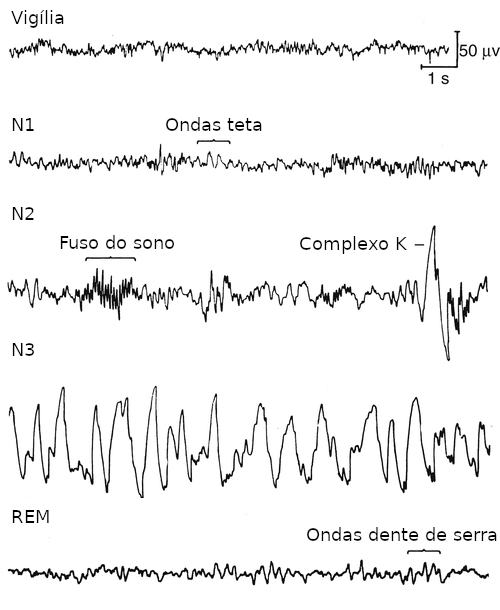
\includegraphics[width=12cm]{figuras/fases_sono.png}
\Fonte{\cite{heuerHeuer2021}. Modificada pelo autor.}
\end{figure}

Durante o sono NREM, as oscilações lentas geradas no córtex promovem uma comunicação bidirecional entre o córtex e o hipocampo,
facilitando a transferência de memórias do hipocampo, onde são inicialmente codificadas, para locais de armazenamento de longo
prazo no neocórtex~\cite{diekelmannMemory2010}. Esta transferência de memórias é suportada pelos fusos do sono que ocorrem durante
a fase N2, que estão associados à plasticidade sináptica e são cruciais para a estabilização das memórias durante o
sono~\cite{raschReactivation2008, peyracheMechanism2020}.

O estágio REM é quando ocorre a maior parte dos sonhos. O sono REM é caracterizado por atividade elétrica cerebral rápida e de
baixa amplitude, similar àquela observada durante o estado de vigília. A dificuldade em isolar a atividade neural dessa etapa
específica, torna a discussão sobre sua contribuição para a consolidação da memória ainda controversa. Contudo, evidências
recentes sugerem que o sono REM também pode facilitar a consolidação da memória espacial e contextual, bem como a regulação
emocional~\cite{payneSleep2012, boyceREM2017}.

A pesquisa sobre a neurobiologia do sono e da memória ainda está em andamento, e ainda não se sabe porque o sono é tão essencial
para a vida em mamíferos, e novas descobertas continuam a esclarecer a complexidade e a importância do sono para a cognição e a
saúde geral.


\chapter{Metodologia}

Nesse capítulo serão apresentados os passos metodológicos para a realização do trabalho, que tem como objetivo principal estudar a
formação e consolidação de memórias em RNPs, com foco em analisar o impacto do sono nesse processo. Para estudar a influência do
sono na formação e recordação de assembleias neu\-ro\-nais foi simulado um modelo de RNP com diferentes formas de plasticidade. A
Figura~\ref{fig_metodologia} apresenta uma visão geral da metodologia, contendo os passos para criação do modelo, que serão
descritos nas seções subsequentes.

\begin{figure}[!ht]
\caption{Visão geral da metodologia: passos para construção do modelo e simulação e análise.}
\centering{
\parbox{12cm}{
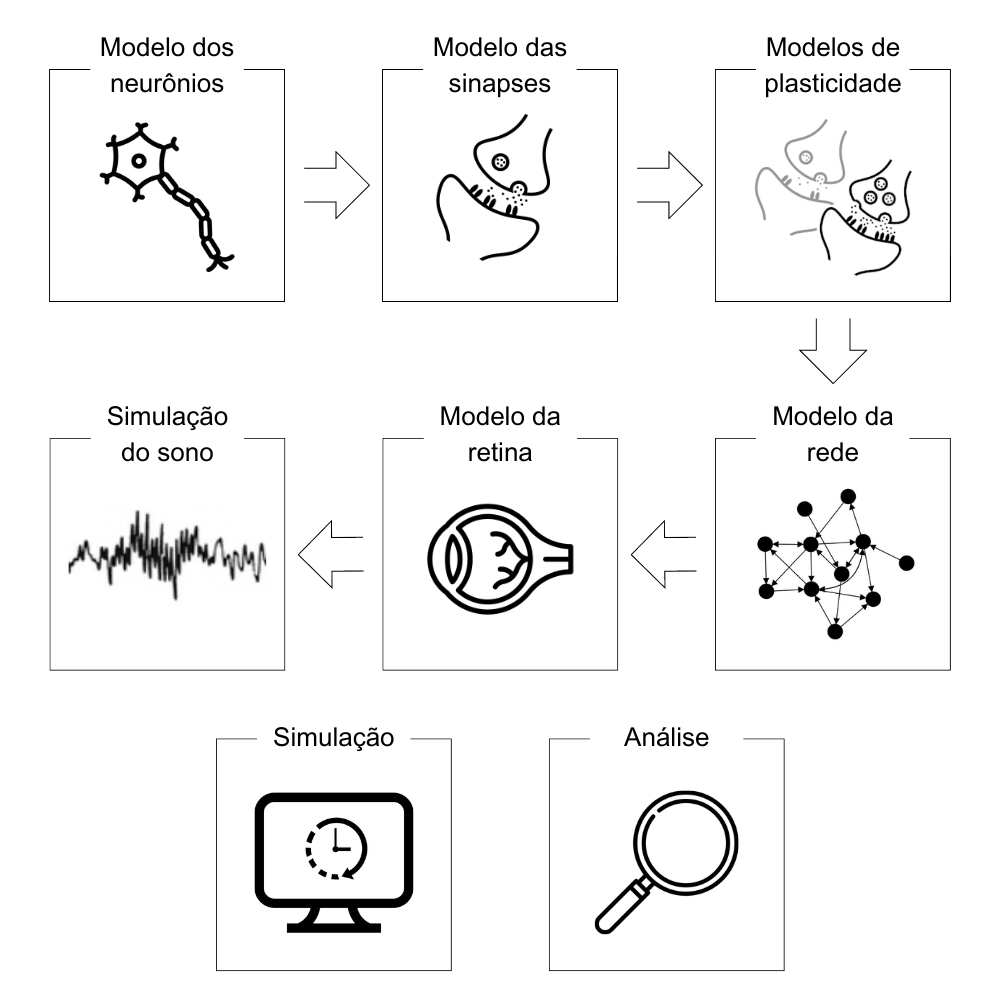
\includegraphics[width=12cm]{figuras/metodologia.png}\label{fig_metodologia}
\fonte{Elaborado pelo autor (2023).}
}}
\end{figure}


\section{Modelo dos neurônios}

A unidade básica de uma RNP é o neurônio, então o primeiro passo para o modelo é a modelagem do neurônio. O modelo de neurônio
utilizado foi o \textit{Leaky Integrate-and-Fire} (LIF) devido à sua simplicidade, que captura o comportamento geral de um
neurônio enquanto permite simulações rápidas de larga escala, como apresentado na Seção~\ref{section_modelos_neuronios}.

O modelo LIF utilizado possui algumas diferenças do descrito na Seção~\ref{section_modelos_neuronios}, pois implementa adaptação
por frequência de disparo\footnote{Comportamento de um neurônio que reduz sua frequência de disparo em resposta a um estímulo
constante.} assim como o trabalho de~\cite{zenkeDiverse2015}, e segue a Equação~\ref{eq_lif_sfa}.

\begin{equation}
\label{eq_lif_sfa}
\tau^m\frac{d}{dt}v_i = (v^{rest} - v_i) + g_i^{exc}(t)(v^{exc} - v_i)+ (g_i^{gaba}(t) + g_i^{a}(t))(v^{ini} - v_i)
\end{equation}

\noindent{}onde $v_i(t)$, $v^{rest}$, $v^{exc}$, $v^{ini}$ se referem, respectivamente, ao potencial de membrana do neurônio,
potencial de repouso, potencial excitatório e potencial inibitório. As condutâncias são descritas por $g_i^{exc}(t)$,
$g_i^{gaba}(t)$, $g_i^{a}(t)$, respectivamente excitatória, inibitória pelos neurônios pré-sinápticos GABAérgicos e inibitória
pela adaptação por frequência de disparo.

\section{Modelo das sinapses}

Para simular como os neurônios interagem entre si, é preciso modelar as sinapses e como as condutâncias apresentadas na seção
anterior evoluem com o tempo. Para isso, foi utilizado o modelo de sinapse de
condução, apresentado na Seção~\ref{subsection_modelos_sinapses}, mas com algumas diferenças notáveis. O comportamento das
condutâncias inibitórias está definido nas Equações~\ref{eq_lif_sfa_ini} e~\ref{eq_lif_sfa_a}:

\begin{equation}
\label{eq_lif_sfa_ini}
\frac{d}{dt}g_i^{gaba} = -\frac{g_i^{gaba}}{\tau^{gaba}} + \sum_{j\in ini}{w_{ij}S_j(t)}
\end{equation}

\begin{equation}
\label{eq_lif_sfa_a}
\frac{d}{dt}g_i^{a} = -\frac{g_i^{a}}{\tau^{a}} + \Delta^{a}S_i(t)
\end{equation}

\begin{equation}
\label{eq_lif_sfa_spikes}
S_j(t) = \sum_{k}{\delta(t-t_j^k)}
\end{equation}

\noindent{}onde $w_{ij}$ refere-se ao peso da sinapse do neurônio $i$ para o $j$. A Equação~\ref{eq_lif_sfa_spikes} representa a
soma de disparos no momento $t$. Nessas equações, a condutância $g$ tende a zero com o tempo, mas quando há um disparo dos
neurônios pré-sinápticos essa condutância sobe, exceto no caso da condutância pela adaptação do neurônio, que aumenta seguindo um
fator $\Delta^{a}S_i(t)$ quando o próprio neurônio dispara.

As sinapses excitatórias são modeladas com um componente rápido AMPA $g_i^{ampa}$ e um componente NMDA $g_i^{nmda}$ que aumenta e
decai lentamente, como detalhado nas Equações~\ref{eq_lif_sfa_exc},~\ref{eq_lif_sfa_ampa} e~\ref{eq_lif_sfa_nmda}:

\begin{equation}
\label{eq_lif_sfa_exc}
g_i^{exc}(t) = \alpha g_i^{ampa}(t) + (1-\alpha)g_i^{nmda}(t)
\end{equation}

\begin{equation}
\label{eq_lif_sfa_ampa}
\frac{d}{dt}g_i^{ampa} = -\frac{g_i^{ampa}}{\tau^{ampa}} + \sum_{j\in exc}{w_{ij} 
\underbrace{u_j(t)x_j(t)}_{\text{PCP}}
S_j(t)}
\end{equation}

\begin{equation}
\label{eq_lif_sfa_nmda}
\tau^{nmda} \frac{d}{dt}g_i^{nmda} = -g_i^{nmda} + g_i^{ampa}
\end{equation}

As conexões excitatórias da RNP também têm a Plasticidade de Curto-Prazo (PCP) simulada pelas variáveis $u_j(t)$ e $x_j(t)$.

Quando $v_i$ utlrapassa seu limiar $\vartheta_i$, o potencial retorna para seu potencial de membrana $v_i^{rest}$. Quando há um
disparo, o limiar aumenta $\vartheta_i \rightarrow \vartheta^{disparo}$ para implementar o período refratário do neurônio, mas na
ausência de disparos, ele retorna lentamente a seu valor usual, como demonstra a Equação~\ref{eq_lif_sfa_thr}:

\begin{equation}
\label{eq_lif_sfa_thr}
\tau^{th}\frac{d\vartheta_i}{dt} = \vartheta^{rest} - \vartheta_i
\end{equation}


\section{Modelos de plasticidade}

As sinapses não são estáticas e têm diversas formas de plasticidade simuladas. As sinapses excitatórias implementam os seguintes
modelos de plasticidade: PCP, PDTD, heterossináptica e a induzida por transmissor, como apresentados na
Seção~\ref{section_modelos_plasticidade}.


\subsection{Plasticidade de curto-prazo}

Como apresentado na seção anterior, as variáveis $u_j(t)$ e $x_j(t)$ controlam a PCP.\@A Equação~\ref{eq_x} descreve a evolução da
fração de recursos sinápticos disponíveis $x_j(t)$ ao longo do tempo, considerando tanto a liberação quanto a recuperação de
neurotransmissores. A Equação~\ref{eq_u} representa a variação na utilização desses recursos $u_j(t)$ com o tempo, refletindo a
probabilidade de liberação de neurotransmissores em resposta a um estímulo. Novamente, $S_j(t)$ indica a presença de um disparo
pré-sináptico, enquanto $\tau^d$ e $\tau^f$ são constantes de tempo que determinam a velocidade de recuperação e decaimento dos
recursos e da sua utilização, respectivamente. O termo $U$ representa a probabilidade básica de liberação de um neurotransmissor em
resposta a um único disparo.

\begin{equation}
\label{eq_x}
\frac{d}{dt} x_j(t) = \frac{1 - x_j(t)}{\tau^d} - u_j(t) x_j(t) S_j(t)
\end{equation}

\begin{equation}
\label{eq_u}
\frac{d}{dt}u_j(t) = \frac{U - u_j(t)}{\tau^f} + U(1 - u_j(t)) S_j(t)
\end{equation}

\subsection{Plasticidade de longo-prazo}

Três tipos de plasticidade de longo-prazo afetam as sinapses excitatórias: PDTD $\mathfrak{P}(t)$ e  $\mathfrak{D}(t)$,
heterossináptica $\mathfrak{H}(t)$ e induzida por transmissor $\mathfrak{T}(t)$. Essas formas de plasticidade afetam diretamente o
peso da sinapse $w_{ij}$, como indica a Equação~\ref{eq_pdtd}:
e~\ref{eq_t}.

\begin{samepage}

\begin{equation}
\label{eq_pdtd}
\frac{d}{dt}w_{ij}(t) = \mathfrak{P}(t) + \mathfrak{D}(t) + \mathfrak{H}(t) + \mathfrak{T}(t)\\
\end{equation}

\begin{align}
\begin{split}\label{eq_p}
  \mathfrak{P}(t) = Az_j^+(t) z_i^{lento}(t - \epsilon)S_j(t){} & \quad\quad\text{PLP tripla}
\end{split}\\
\begin{split}\label{eq_d}
  \mathfrak{D}(t) = - B_i(t)z_i^- (t)S_j(t){} & \quad\quad\text{DLP dupla}
\end{split}\\
\begin{split}\label{eq_h}
  \mathfrak{H}(t) = - \beta (w_{ij} - \bar{w}_{ij}(t)) (z_i^- (t - \epsilon))^3 S_i(t){} & \quad\quad\text{Heterossináptica}
\end{split}\\
\begin{split}\label{eq_t}
  \mathfrak{T}(t) = \delta S_j(t){} & \quad\quad\text{Induzida por transmissor}
\end{split}
\end{align}

\end{samepage}

As Equações~\ref{eq_p} e~\ref{eq_d} representam a potenciação e a depressão de longo-prazo, respectivamente, usando uma regra
tripla, ou seja, que leva em consideração 3 disparos~\cite{pfisterTriplets2006}. Os parâmetros $A$, $\beta$ e $\delta$ são apenas
escalares fixos, assim como $B_i(t)=A$. A variável $z_k^x(t)$ representa os traços sinápticos dos neurônios pré- (índice $j$) e
pós-sinápticos (índice $i$), e ela evolui de acordo com a Equação~\ref{eq_z}:

\begin{equation}
\label{eq_z}
\frac{d}{dt}z_i^x(t) = - \frac{z^x}{\tau^x}+S_i(t)
\end{equation}

\noindent{}em que $x$ pode tomar diferentes valores representando diferentes traços sinápticos. As variáveis $z^+$ e $z^-$
representam traços de atividade neuronal associados à potenciação e depressão sináptica, respectivamente. Quando um neurônio
pré-sináptico dispara antes de um pós-sináptico, isso pode levar ao aumento da força sináptica, relacionado ao traço $z^+$.
Inversamente, se o neurônio pós-sináptico dispara antes, a força sináptica pode diminuir, associado ao traço $z^+$. Já $z^{lento}$
refere-se a um traço que decai lentamente, capturando a atividade neuronal ao longo de um período de tempo mais extenso.

\subsubsection{Plasticidade de longo-prazo em sinapses inibitórias}

Também seguindo o modelo de~\citeonline{zenkeDiverse2015}, as sinapses inibitórias são moduladas pela PDTD hipotética descrita na
Equação~\ref{eq_pdtd_ini}, que basicamente tende a potencializar as sinapses inibitórias quando a atividade excitatória global da
rede estiver muito alta: 

\begin{equation}
\label{eq_pdtd_ini}
\frac{d}{dt}w_{ij}(t) = \eta G(t) [(z_i(t) + 1) S_j(t) + z_j(t) S_i(t)]
\end{equation}

\noindent{}onde $\eta$ é uma constante, $z_k$ representa os traços sinápticos e $G(t) = H(t) - \gamma$, em que $H(t)$ é o fator
global secretado, um valor que comprime toda a atividade do grupo excitatório e evolui segundo a Equação~\ref{eq_pdtd_ini_h} :

\begin{equation}
\label{eq_pdtd_ini_h}
\frac{d}{dt}H(t) = - \frac{H(t)}{\tau^H} + \sum_{i \in \text{exc}} S_i(t)
\end{equation}

Quando a atividade global da população excitatória $H(t)$ cai abaixo de um valor-alvo $\gamma$, $G(t)$ é menor que zero e a regra
de aprendizagem da Equação~\ref{eq_pdtd_ini} se torna uma regra unidirecional de "depressão". Se a atividade da rede for maior que
$\gamma$, a regra de aprendizagem se torna hebbiana. Isso serve para estabilizar a dinâmica geral da rede.

\section{Arquitetura da rede}

A rede é estruturada com um total de 5.120 neurônios do tipo LIF, distribuídos em dois grupos principais. O primeiro grupo é
formado por 4.096 neurônios excitatórios, enquanto o segundo grupo contém 1.024 neurônios inibitórios. Além disso, há grupos
auxiliares como a retina (Detalhada na Seção~\ref{subsection_retina}) e o grupo responsável pelos padrões de sono (Detalhado na
Seção~\ref{subsection_sono}). Para as conexões entre o grupo excitatório e inibitório, cada neurônio é conectado a 10\% dos
neurônios de outro grupo ou do seu próprio grupo, e essa conectividade é estabelecida de forma aleatória. As conexões excitatórias
entre neurônios são moduladas pelo neurotransmissor glutamato, com receptores AMPA e NMDA, enquanto as conexões inibitórias são
moduladas pelo neurotransmissor GABA.

\subsection{Modelo da retina}\label{subsection_retina}

De modo a simular a entrada de estímulos visuais, foi simulada uma retina. A retina é composta de 4.096 neurônios LIF, com cada
neurônio representando um pixel em uma imagem de 64$\times$64 pixels. Cada neurônio excitatório da RNP recebe conexões dos
neurônios da retina de uma área circular de raio 8, em que o centro do círculo é escolhido aleatoriamente para cada neurônio, como
exemplifica a Figura~\ref{fig_estimulo_raio}. As conexões da retina com a RNP também são plásticas.

\begin{figure}[!ht]
\caption{Exemplo de estímulo apresentado à RNP.\@Aqui, um neurônio com seu campo receptivo centralizado no X recebe conexões dos neurônios da retina contidos dentro da grade verde.}
\centering{
\parbox{6cm}{
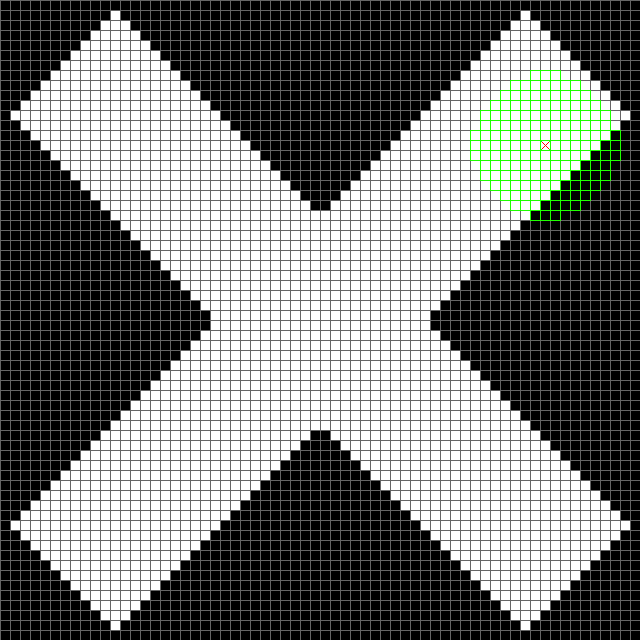
\includegraphics[width=6cm]{figuras/estimulo_raio.png}\label{fig_estimulo_raio}
\fonte{Elaborado pelo autor (2023).}}}
\end{figure}

Como explicado na Seção~\ref{section_experimento}, são utilizados 6 estímulos diferentes, que são imagens simples de serem
reconhecidas, como formas geométricas e símbolos. Essas imagens são binárias: apenas preto e branco; o neurônio da retina
correspondente a um pixel preto irá disparar com frequência média de 10Hz, enquanto o neurônio correspondente a um pixel branco
irá disparar com frequência média de 35Hz, ou seja, com uma maior ativação.

\subsection{Simulação do sono}\label{subsection_sono}

Para simular o sono, a rede funciona de dois modos diferentes intercalados: um modo de atividade ou vigília, em que a rede
funciona normalmente enquanto recebe estímulos, e um modo de inatividade ou sono, em que será simulado o sono. 

Durante o ciclo de sono, nenhum estímulo é apresentado à rede, contudo, ela continua sendo simulada normalmente. Essa etapa é
subdividida em duas fases, correspondentes às fases do sono real: REM e NREM. Em um ciclo completo de sono, as fases REM e NREM se
alternam, iniciando-se com a fase NREM, seguida pela REM, sendo que cada uma destas fases ocupa um oitavo da duração total do
sono. Assim, o ciclo de NREM e REM se repete quatro vezes em um ciclo completo de sono, de maneira análoga ao que ocorre nos
humanos, nos quais cada noite de sono compreende entre 4 a 6 ciclos~\cite{patelPhysiology2023}.

Para simular cada fase do sono, é utilizado um grupo de 256 neurônios excitatórios que se ativam de maneira sinusoidal e
conectam-se a 20\% dos neurônios do grupo de neurônios excitatórios. Durante a fase NREM, a frequência dessa onda de ativação
sinusoidal é de 1Hz, enquanto na fase REM é de 16Hz, visando aproximar-se, de forma simplificada, das frequências observadas
durante essas fases em humanos~\cite{guoSlow2022, cowdinTheta2014}. Este método foi inspirado no trabalho de~\citeonline{bazhenovModel2002}, que
simulou o sono de maneira similar, utilizando um grupo de neurônios com 25\% de conectividade com a rede, com um disparo médio de
25Hz modulados por uma função sinusoidal.

\subsection{Análise de assembleias neuronais}

A parte final do trabalho consiste em analisar as diferentes simulações realizadas e determinar se a simulação de sono teve algum
efeito na formação de assembleias neuronais. Para isso, antes de tudo é necessário definir um modo de identificar as assembleias
neuronais e quais neurônios pertencem a cada uma.

Para determinar quais neurônios pertencem à assembleia neuronal associada a um estímulo, o método consiste em analisar a
frequência de disparos de cada neurônio no intervalo $3s < t < 3.5s$ após a apresentação do estímulo. Os neurônios que disparam
com frequência maior que 20Hz nesse intervalo são considerados como pertencentes à assembleia neuronal associada a esse estímulo.
No trabalho de~\citeonline{zenkeDiverse2015} foram analisados os neurônios com frequência de disparos maior que 10Hz, mas nesse
trabalho optou-se por considerar apenas os com frequência maior que 20Hz, pois com esse valor a soma total de todos os neurônios
em assembleias neuronais chegou mais próximo do número total de neurônios da rede, incluindo neurônios repetidos em cada
assembleia.

\subsection{Detalhes da simulação}

A simulação foi feita em C++ utilizando o framework Auryn~\cite{zenkeLimits2014}.

\chapter{Experimentos}\label{section_experimento}

Como forma de avaliar o modelo proposto serão conduzidos dois principais experimentos.

\section{Experimento 1: Formação de assembleias neuronais}

O primeiro experimento consiste em simular a RNP apresentando estímulos ao modelo de retina e analisar se a repetição dos
estímulos leva à formação de assembleias neuronais associadas a cada estímulo a longo prazo, com o objetivo de ter uma base de
comparação para o experimento 2, que terá o sono simulado. Os estímulos consistem em seis imagens simples de serem reconhecidas,
exibidas na Figura~\ref{fig_estimulos}, e são apresentados à rede de forma intercalada e aleatória. Quatro estímulos foram
reaproveitados do trabalho de~\citeonline{zenkeDiverse2015}, enquanto as figuras de diamante e de cruz foram adicionadas com o
intuito de colocar a RNP mais próxima do seu limite.

\begin{figure}[!ht]
\caption{Os seis estímulos apresentados à RNP durante os experimentos.}
\centering{
\parbox{12cm}{
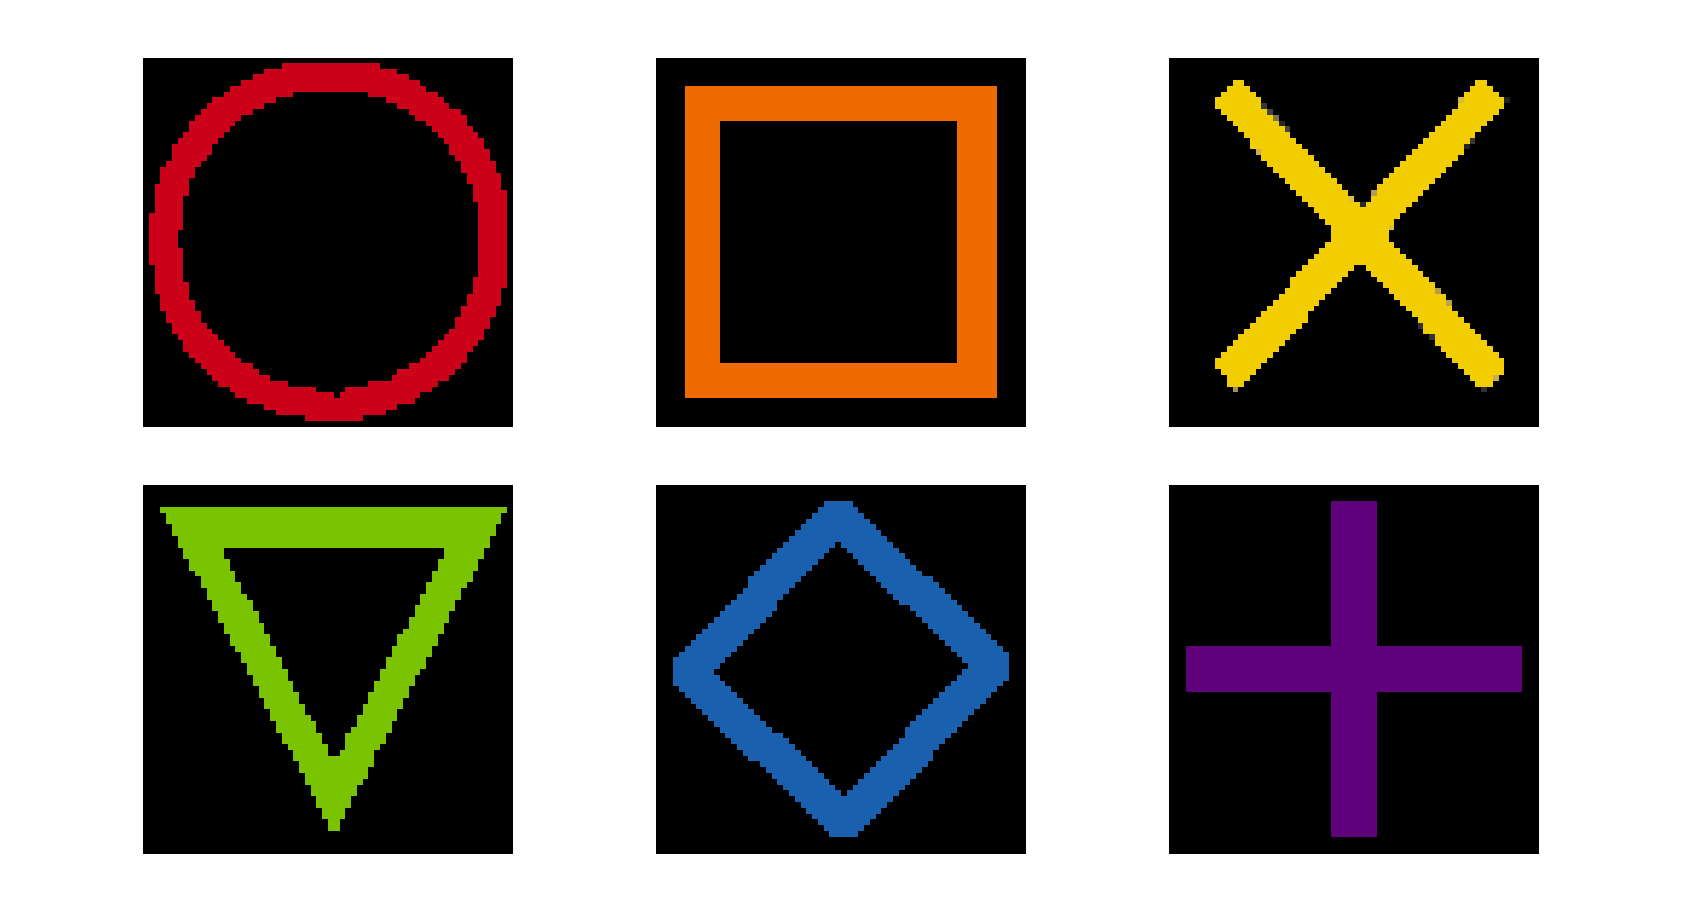
\includegraphics[width=12cm]{figuras/estimulos_cor.png}\label{fig_estimulos}
\fonte{Elaborado pelo autor (2023).}}}
\end{figure}

Houveram três fases da simulação da RNP:

\begin{enumerate}
  \item Simulação da rede em seu estado inicial por 1800 segundos, com um tempo médio de aparição do estímulo de 2 segundos, e
  tempo médio entre estímulos de 1 segundo. O peso das sinapses entre a retina e a rede é de 0.05.
  \item Simulação da rede também por 1800 segundos, mas com um tempo médio de aparição do estímulo de 0.2 segundo, e
  tempo médio entre estímulos de 5 segundos. O peso das sinapses entre a retina e a rede agora é de 0.1. A intenção aqui é
  fazer com que a rede tenha mais tempo entre um estímulo e outro para poder memorizá-los melhor.
  \item A última simulação é de 2400 segundos e é de onde são tirados os resultados. O tempo médio de aparição do estímulo diminui
  para 0.1, enquanto o tempo médio entre estímulos é de 10 segundos, com a intenção de ter uma janela maior de tempo entre os
  estímulos para analisar a capacidade de memorização da RNP.
\end{enumerate}


\section{Experimento 2: Formação de assembleias neuronais com sono}

De forma similar ao experimento 1, o segundo experimento consiste em simular a RNP apresentando os mesmos estímulos, mas dessa vez
com a simulação de sono. O objetivo desse experimento é analisar se a simulação de sono tem algum efeito na formação de
assembleias neuronais.

Esse experimento seguiu as mesmas três fases do experimento anterior, mas com a simulação do sono. Nesse experimento, a RNP ficava
em estado de vigília por 200s e dormia por 100s, seguindo uma proporção similar a de humanos que ficam acordados 16 horas por dia
e dormem 8~\cite{waterhouseDaily2012}.

\section{Análise dos resultados}

\subsection{Formação de assembleias neuronais}

O número médio de neurônios por assembleia neuronal na RNP base foi de 787, enquanto na RNP com sono foi de 432.67; isso se deve
principalmente ao fato de que as assembleias neuronais do círculo e do quadrado tiveram pouquíssimos neurônios, apenas 42 e 34 na
RNP com sono. Ambas as RNPs tiveram dificuldades em manter uma assembleia neuronal única para o estímulo do círculo, havendo
bastante sobreposição com os neurônios da assembleia neuronal do quadrado; isso provavelmente ocorre pela similaridade entre os
dois estímulos e também a possibilidade da RNP ter alcançado um limite de memória. A matriz de sobreposição das assembleias
neuronais está ilustrada nas Figura~\ref{fig_mat_base}.

\begin{figure}[!ht]
\caption{Matrizes contendo o número de neurônios pertecentes a cada assembleia neuronal. Os elementos da diagonal principal da
matriz indicam o número total de neurônios em cada assembleia individual. Nos outros casos, o elemento representa quantos
neurônios de uma assembleia também são parte de outra assembleia.}

\centering{
\parbox{\linewidth}{
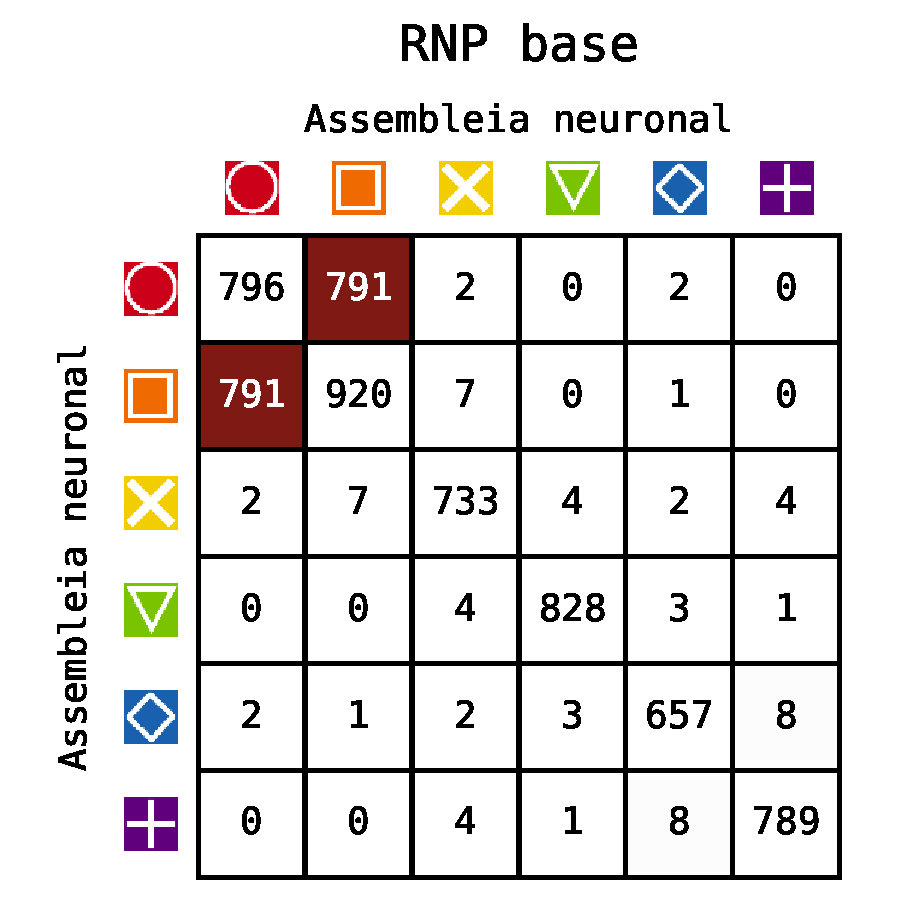
\includegraphics[width=7.5cm]{figuras/plots_pdf/RNP base.pdf}\label{fig_mat_base}
\hfill
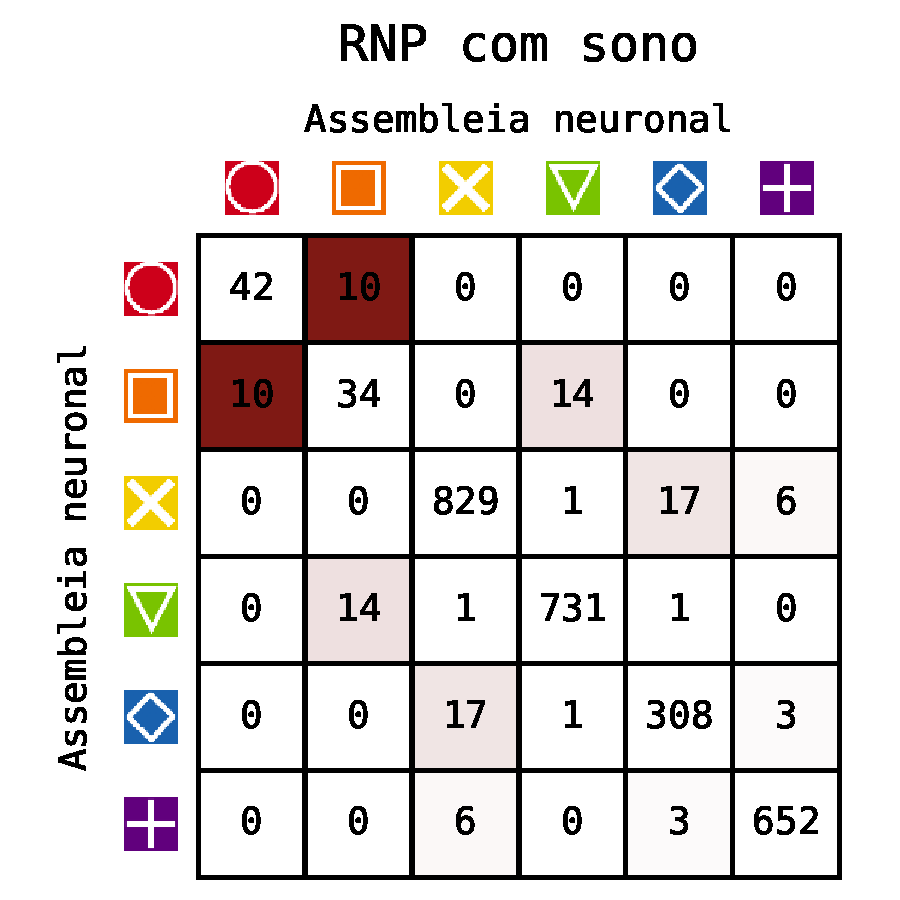
\includegraphics[width=7.5cm]{figuras/plots_pdf/RNP com sono.pdf}\label{fig_mat_sleep}
\fonte{Elaborado pelo autor (2023).}}}
\end{figure}

Outra forma de analisar o comportamento das RNPs é verificando a ativação média das assembleias neuronais para cada estímulo, como
mostra a Figura~\ref{fig_mat_act_base}. A diagonal principal claramente possui as maiores médias pois a assembleia neuronal de um
determinado estímulo vai apresentar muito mais atividade para esse estímulo. Nota-se também que na RNP com sono houve mais
atividade nas assembleias neuronais não relacionadas com o estímulo, indicando uma piora na performance.

\begin{figure}[!ht]
\caption{Matrizes representando a ativação média em Hz de cada assembleia neuronal para cada estímulo diferente.}
\centering{
\parbox{\linewidth}{
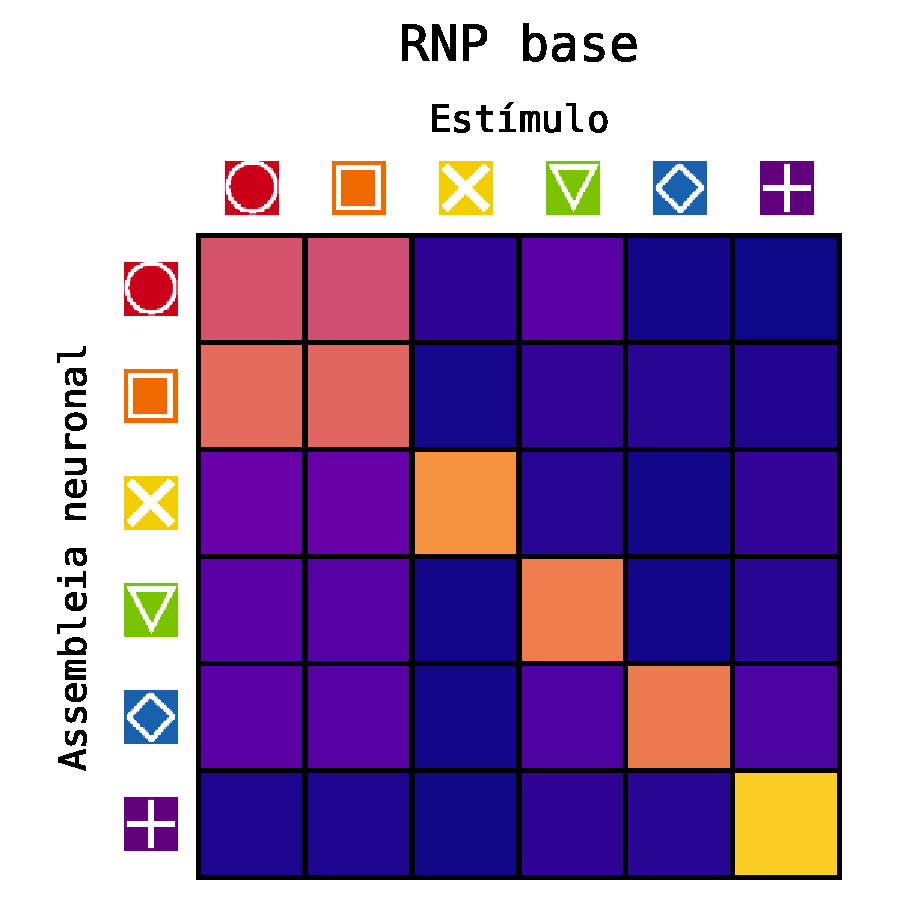
\includegraphics[height=7cm]{figuras/plots_pdf/RNP base_atv.pdf}\label{fig_mat_act_base}
\hfill
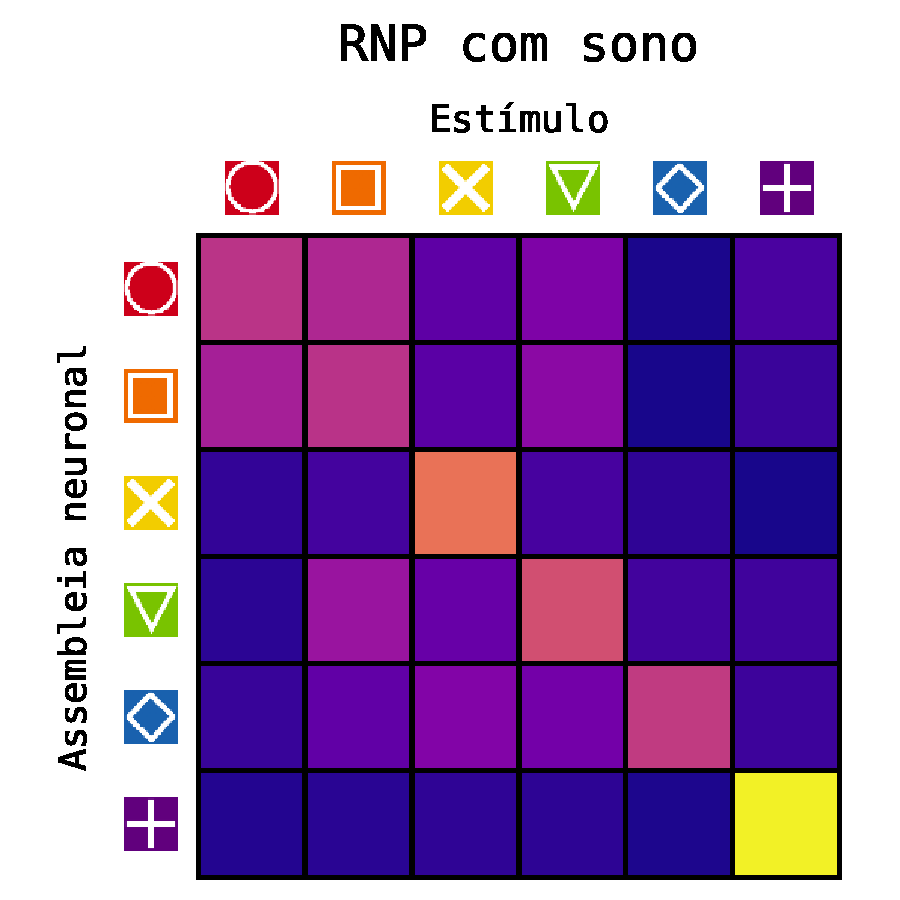
\includegraphics[height=7cm]{figuras/plots_pdf/RNP com sono_atv.pdf}\label{fig_mat_act_sono}
\hfill
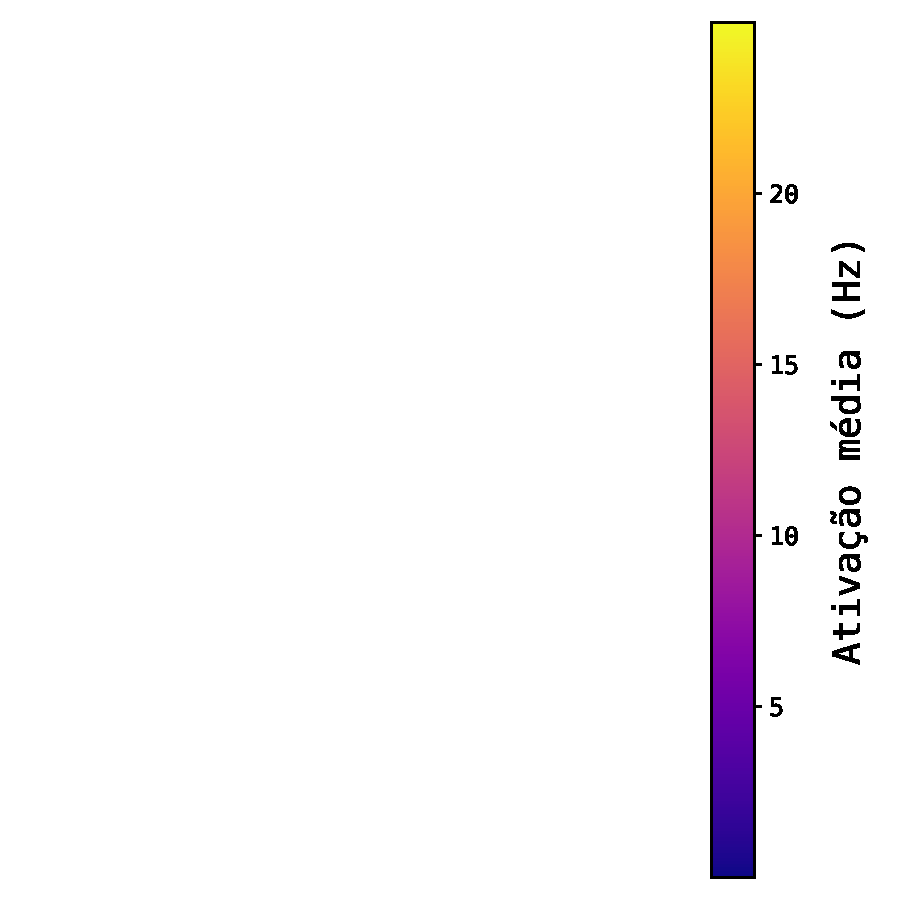
\includegraphics[height=5.8cm]{figuras/plots_pdf/atv_colorbar.pdf}\label{fig_mat_act_colorbar}
\fonte{Elaborado pelo autor (2023).}}}
\end{figure}

Com base nesses resultados, pode-se deduzir que a simulação do sono não afetou significativamente a formação de assembleias
neuronais, ou que no máximo serviu apenas para limitar as capacidades da rede.

\subsection{Atividade da RNP}

Outra forma de analisar os resultados da simulação é analisando diretamente os dados dos disparos dos neurônios. A
Figura~\ref{fig_base_act} contém um gráfico relacionando o momento dos estímulos (topo da figura) com a ativação média das
assembleias neuronais (parte inferior da figura). É possível identificar que na maioria das vezes em que um estímulo é apresentado
à RNP, a assembleia neuronal associada a esse estímulo dispara e mantém-se ativa até que outro estímulo domine a atividade da
RNP;\@é importante notar que o estímulo é mostrado para a RNP por menos de 1 segundo, portanto a ativação da assembleia neuronal
nos segundos seguintes é a memória do estímulo.

Também pode-se notar que quando é mostrado o estímulo do círculo ou do quadrado, as assembleias neuronais de ambos os estímulos
disparam juntas, devido à sobreposição de neurônios entre as duas assembleias neuronais\footnote{Se é que podem ser consideradas
duas assembleias neuronais, já que os neurônios são quase todos os mesmos em ambas.} identificada na seção anterior.

\begin{figure}[!ht]
\caption{Ativação das assembleias neuronais na simulação da RNP base.}
\centering{
\parbox{\linewidth}{
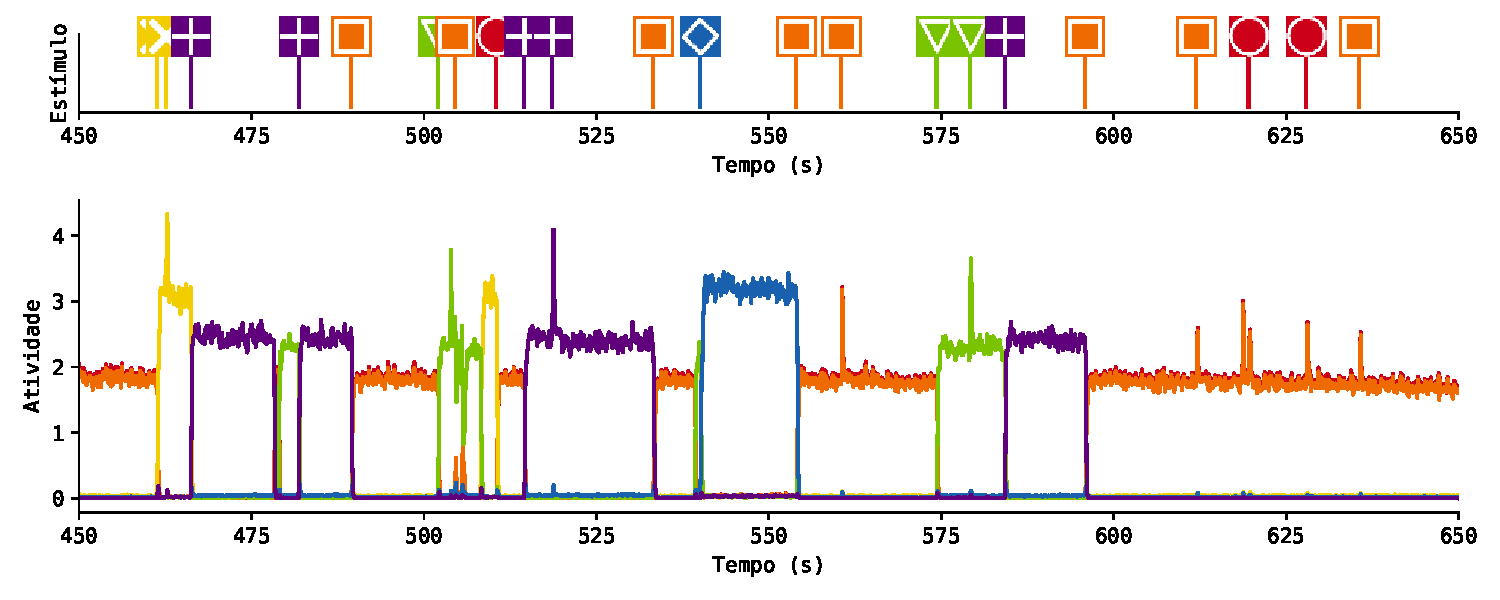
\includegraphics[width=\linewidth]{figuras/plots_pdf/atividade base.pdf}\label{fig_base_act}
\fonte{Elaborado pelo autor (2023).}}}
\end{figure}

Durante as simulações de sono da RNP, em diversas instâncias foram observados padrões intrigantes de atividade, como ilustrado nas
Figuras~\ref{fig_sleep_act} e~\ref{fig_sleep_act2}. Em várias casos, ao entrar no modo de sono, a RNP mantém uma atividade
consistente de uma assembleia neuronal, correspondente à resposta ao último estímulo mostrado a ela. Esta atividade é sustentada
por algum tempo, no entanto, há um momento em que ela diminui e é substituída por uma nova assembleia neuronal que emerge com uma
série de disparos. Como uma assembleia neuronal é a representação de uma memória na RNP, essa reativação da assembleia neuronal
representa um momento durante o sono em que a RNP se recorda de algum estímulo.

\begin{figure}[!ht]
\caption{Ativação das assembleias neuronais na simulação da RNP com sono em momento de ``sonho''. A cor cinza indica o período de sono.}
\centering{
\parbox{\linewidth}{
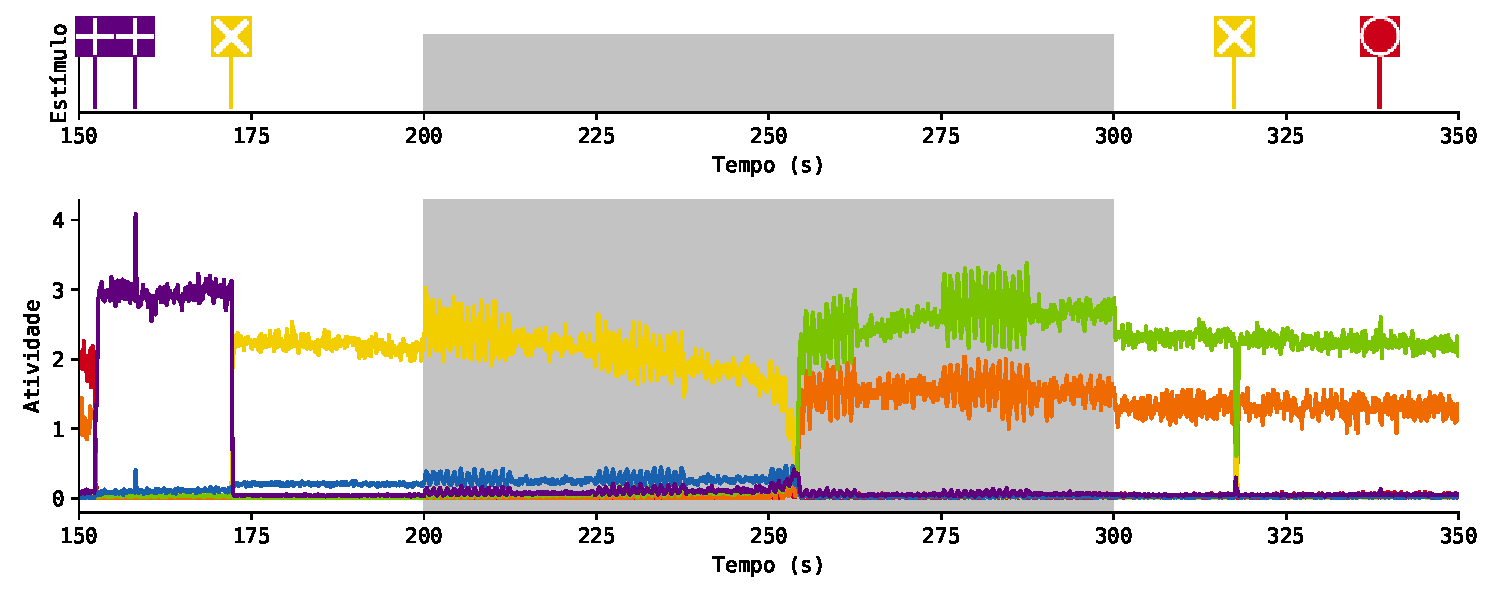
\includegraphics[width=\linewidth]{figuras/plots_pdf/atividade sonho1.pdf}\label{fig_sleep_act}
\fonte{Elaborado pelo autor (2023).}}}
\end{figure}

\begin{figure}[!ht]
\caption{Ativação das assembleias neuronais na simulação da RNP com sono em outro momento de ``sonho''. A cor cinza indica o período de sono.}
\centering{
\parbox{\linewidth}{
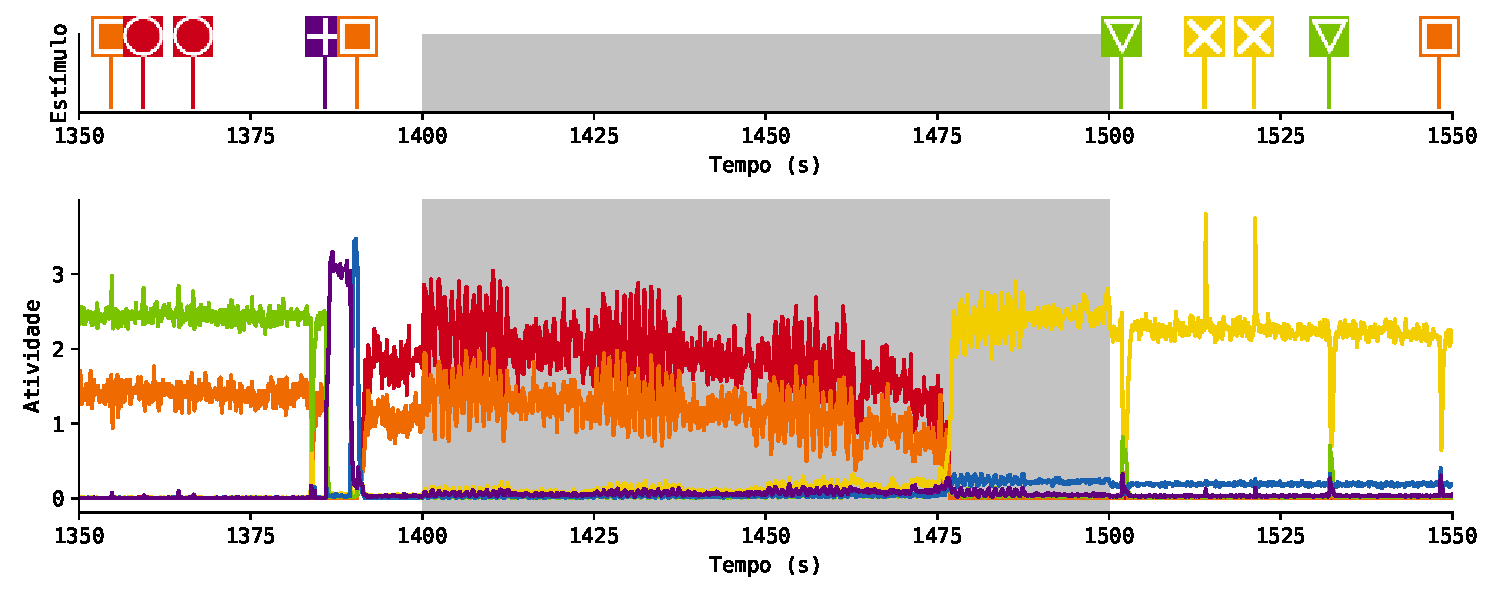
\includegraphics[width=\linewidth]{figuras/plots_pdf/atividade sonho2.pdf}\label{fig_sleep_act2}
\fonte{Elaborado pelo autor (2023).}}}
\end{figure}

Esse padrão de reativação da assembleia neuronal pode ser interpretado analogamente aos processos de sonho em organismos
biológicos. Segundo o trabalho de~\citeonline{picard-delandMemory2023}, existe um fenômeno observado durante o sono em que rastros
de memória recém-formados são reativados espontaneamente durante o sono, e esse fenômeno pode ou não estar conectado com a experiência de
sonhos e com a consolidação de memórias durante o sono.

No entanto, é fundamental abordar esta interpretação com cautela. Embora as semelhanças sejam intrigantes, é essencial
não tirar conclusões precipitadas e reconhecer que mais pesquisas são necessárias antes de afirmar que esses padrões representam
efetivamente ``sonhos'' em RNP.\@


\chapter{Resultados esperados}

Espera-se que a análise do modelo de RND implementado possa contribuir para o entendimento dos mecanismos subjacentes aos
processos de aprendizado e memória no cérebro, principalmente a influência do sono sobre isso. Além disso, espera-se que a
simulação das fases do sono possa melhorar a consolidação e retenção de memórias na RND, possibilitanto que a rede seja capaz de
aprender mais estímulos, por mais tempo e até esquecer estímulos não mais relevantes.

\section{Considerações finais}

Ao longo deste trabalho, foram explorados os aspectos teóricos do desenvolvimento e da aplicação das Redes Neurais de Disparos
(RNDs) para entender melhor a formação e consolidação de memórias no cérebro humano. A principal questão abordada foi a
possibilidade de simulações de fases do sono melhorarem a estabilidade e formação de assembleias neuronais, contribuindo para a
retenção de memórias. 

No entanto, este trabalho se concentrou na parte teórica dessas questões. O próximo passo, na continuação desse trabalho, será
implementar e aplicar um modelo que empregue as ideias discutidas aqui e analisar as implicações de simulações do sono em tal
modelo neural.

Por fim, vale salientar que este trabalho posiciona-se na intersecção crucial entre a neurociência computacional e a inteligência
artificial. Ao iluminar os processos subjacentes à formação e consolidação da memória no cérebro humano e o papel do sono nisso,
estamos expandindo a fronteira de nossa compreensão na neurociência. Além disso, ao melhorar nossa capacidade de simular esses
processos em modelos de RNDs, também estamos avançando na área de inteligência artificial, aprofundando nossa compreensão de como
a inteligência pode ser replicada e potencialmente aperfeiçoada. 


% \chapter{Conclusão}

	
% Elementos pós-textuais

\bibliography{elementos_pos_textuais/referencias}
%\imprimirglossario	
%\imprimirapendices
%\apendice{Exemplo de Apêndice}

\begin{quadro}[!ht]	
\centering
\Caption{\label{qua:exemplo-2} Normas técnicas vigentes sobre normalização de trabalhos acadêmicos do ABNT/CB - 014}
\IFCEqua{}{
\begin{tabular}{|c|c|}
\hline
\textbf{Número} & \textbf{Título} \\
\hline
6022:2018 & Artigo em publicação periódica técnica e/ou científica - Apresentação \\
\hline
6023:2002 & Referências - Elaboração \\
\hline
6024:2012 & Numeração progressiva das seções de um documento - Apresentação \\
\hline
6027:2012 & Sumário - Apresentação \\
\hline
6028:2003 & Resumo - Apresentação \\
\hline
6034:2004 & Índice - Apresentação \\
\hline
10520:2002 & Citações em documentos - Apresentação \\
\hline
10719:2015 & Relatório técnico e/ou científico - Apresentação \\
\hline
12225:2004 & Lombada - Apresentação \\
\hline
14724:2011 & Trabalhos acadêmicos - Apresentação \\
\hline
15287:2011 & Projeto de pesquisa - Apresentação \\
\hline
15437:2006 & Pôsteres técnicos e científicos - Apresentação \\
\hline
\end{tabular}
}{
\Fonte{elaborado pelo autor, de acordo com o Catálogo da ABNT.}
}
\end{quadro}
%\imprimiranexos
%\anexo{Exemplo de Anexo}

\begin{center}
\begin{figure}[!ht]
\centering
%\Caption{\label{fig:exemplo-2}xxx}	
\IFCEfig{}{
\fbox{
\includegraphics[width=2.5cm]{figuras/brasao-brasil}}
}{
%\Fonte{xxx}
}	
\end{figure}
\vspace*{-0.8cm}
\textbf{
SERVIÇO PÚBLICO FEDERAL \\
INSTITUTO FEDERAL DE EDUCAÇÃO, CIÊNCIA E TECNOLOGIA CATARINENSE \\
CONSELHO SUPERIOR
}
\end{center}

\begin{center}
\textbf{RESOLUÇÃO N° 01, DE 10 DE JANEIRO DE 2018}
\end{center}

\vspace*{-1cm}

\begin{SingleSpace}
\begin{flushright}
\begin{minipage}[b]{8cm}
\begin{small}
Aprova \textit{ad referendum} a criação do curso Superior de Tecnologia em Gestão Ambiental no \textit{campus} Paracuru. 
\end{small}
\end{minipage}
\end{flushright}
\end{SingleSpace}

\textbf{O PRESIDENTE EM EXERCÍCIO DO CONSELHO SUPERIOR DO INSTITUTO FEDERAL DE EDUCAÇÃO, CIÊNCIA E TECNOLOGIA CATARINENSE}, no uso de suas atribuições legais e estatutárias e considerando o Memorando n$^{\circ}$ 001/2018/GDG da direção-geral do campus Paracuru, 

\textbf{RESOLVE:}

\textbf{Art. $1^{\circ}$} - Criar, \textit{ad referendum} do Conselho Superior, o curso Superior de Tecnologia em Gestão Ambiental do \textit{campus} Paracuru e autorizar a oferta de 35 vagas semestrais.

\textbf{Parágrafo único} - O curso será ofertado na modalidade presencial e nos turnos matutino e vespertino, conforme definido no projeto pedagógico em anexo. 

\textbf{Art. $2^{\circ}$} - A interrupção da oferta e/ou a extinção do referido curso deverá ser submetida a este conselho para aprovação, com as devidas justificativas e a apresentação do planejamento de realocação de recursos humanos e de materiais vinculados ao curso.

\begin{center}
José Wally Mendonça Menezes \\
\textbf{Presidente em exercício do Conselho Superior}
\end{center}		
%\imprimirindice

\end{document}